\chapter{数据库环境的准备}
本章主要记录如何准备各种目标数据库,其中着重记录了 Oracle 11g R2 的安装以及配置。因为它总是如此让人捉摸不透。

\section{Oracle 11g R2 环境的安装和使用}
近期可获取的 Oracle 的最老版本为 11g R2,安装之前可以先去 Oracle 官网下载该版本的数据库。

准备条件:\footnote{本节中的内容全部在 Linux 环境,不考虑 Windows 的兼容性。}

\begin{itemize}
\item 一个带桌面环境的 Linux 发行版,将其作为宿主机器,你需要它的 X 环境来点击 Oracle 安装过程中的各种按钮。
    %\begin{quote}
    %    when install oracle in Centos, you may need to install X11:
    %        
    %    \begin{lstlisting}
    %        yum groupinstall basic-desktop desktop-platform x11 fonts
    %    \end{lstlisting}

    %    Then edit {\ff /etc/inittab}, change {\cf id:3:initdefault:} to {\cf id:5:initdefault:} to start X at boot-up
    %\end{quote}

\item Oracle 专用的 Linux 发行版,推荐 {\ff OracleLinux-R6-U5-Server-x86\_64-dvd.iso},如果需要其它版本,到\href{http://mirrors.wimmekes.net/pub/iso/}{这里}下载。

\item Oracle 11g R2,到 Oracle 官网下载两个文件 {\ff linux.x64\_11gR2\_database\_1of2.zip} 和 {\ff linux.x64\_11gR2\_database\_2of2.zip}。

\item Oracle 的 instant client,到 Oracle 官网下载 {\ff instantclient-basic-linux-12.1.0.1.0.zip} 和 {\ff instantclient-sqlplus-linux-12.1.0.1.0.zip}。\footnote{我下载的大版本号是 12,其实它是兼容服务器端的 11 版本号。如果碰到问题,请直接下载其版本为 11 的客户端。}
\end{itemize}

如果没有实体机器,就用 Virtualbox 虚拟几个,一个用于安装 Oracle Linux,一个用于安装客户端,客户端推荐使用 Linux,可以用 Ubuntu,为节约性能,直接使用不带 UI 的 Ubuntu 即可,如 {\ff ubuntu-12.04.4-server-amd64.iso};但对服务器端而言,最好选择 Oracle 自己的 Linux 发行版,其它版本的 Linux 虽然也可以安装 Oracle,但说多了都是泪,直接用 Oracle 自己的 Linux 发行版是最好的选择。

在 Virtualbox 中安装这两个 Linux 系统,如果可以,将服务器的内存尽量放大一点(2G+)。安装完后,将两个虚拟机的 IP 设置为桥接模式,重启网络后\footnote{\cf /etc/init.d/network restart},这样它们与宿主机就处于同一网段,假定 Oracle Linux 的 IP 为 {\cf 192.168.37.194},Ubuntu 客户机的 IP 为 {\cf 192.168.37.193}。

\begin{quote}
有时候安装的 Oracle Linux 只能使用环回地址(lo),用 {\cmdf ifconfig -a} 查看后,确实有 {\cf eth0},此时需要启动一下该网卡,并设置其通过 DHCP 获取 IP 地址。

    \begin{lstlisting}
    ifconfig eth0 up
    # 在 /etc/sysconfig/network-scripts/ifcfg-eth0 中
    DEVICE=eth0
    BOOTPROTO=dhcp
    ONBOOT=yes
    # 然后重新启动 eth0
    ifup eth0
    \end{lstlisting}

\end{quote}

接下来将下载的 Oracle 数据库安装文件拷贝到 194,将 instantclient 拷贝到 193。分别以 SSH 登录到这两台机器。

\begin{lstlisting}
xhost +192.168.37.194 # 设定 X 服务,使得 194 可以访问 host 上的 X 服务
ssh -X 192.168.37.194
ssh -X 192.168.37.193
\end{lstlisting}

由于两个虚拟机都不带桌面环境,所以此处用 {\cf -X} 选项,使得它们可以访问宿主机上的桌面环境。

在 Oracle Linux 上安装 Oracle 11g R2,参见\href{http://www.oracle-base.com/articles/11g/oracle-db-11gr2-installation-on-oracle-linux-6.php}{这里}的详细步骤。

然后安装客户端,将两个 zip 文件解压后,会得到目录 {\ff instantclient\_12\_1},然后设置两个环境变量 {\cf PATH} 和 {\cf LD\_LIBRARY\_PATH},将它们指向该目录。

接下来在 {\cf instantclient\_12\_1} 中,编辑两个文件。第一个为 {\ff sqlnet.ora},在其中加入如下内容

\begin{lstlisting}
QLNET.AUTHENTICATION_SERVICES= (NTS)
NAMES.DIRECTORY_PATH= (TNSNAMES, EZCONNECT)
\end{lstlisting}

第二个文件为 {\ff tnsnames.ora},在其中加入如下内容

\begin{lstlisting}
databasename =
(DESCRIPTION =
 (ADDRESS_LIST =
  (ADDRESS = (PROTOCOL = TCP)(HOST = 192.168.37.194)(PORT = 1521))
 )
 (CONNECT_DATA =
  (SERVICE_NAME = orcl11g)
 )
 )
\end{lstlisting}

为便于连接 194 上的数据库,编写脚本 {\ff login-oracle.sh}:

\begin{lstlisting}
sqlplus system/test@'(DESCRIPTION=(ADDRESS=(PROTOCOL=TCP) \
  (HOST=192.168.37.194)(PORT=1521))(CONNECT_DATA=(SID=orcl11g)))'
\end{lstlisting}

客户端配置完毕,此时你应该可以在命令行执行该登录脚本。但是登录不会成功。

接下来配置服务器端,由于 Oracle Linux 默认开启了多个 iptables 的防火墙设置,所以需要将它们一一关闭,登录 194:

\begin{lstlisting}
service iptables save
service iptables stop
chkconfig iptables off

service ip6tables save
service ip6tables stop
chkconfig ip6tables off
\end{lstlisting}

这样,在 193 上应该就能访问 194 上的服务了。

当下一次服务器重启的时候,可能你什么都找不到了,但是没关系,上面的链接中给了很多设定,最重要的是环境变量,没记错的话,应该都放到用户目录的 {\ff .bash\_profile} 中去了。如果下一次启动的时候,这些环境变量都没了(典型的表现是输入 {\cmdf sqlplus} 说找不到这个命令),那么在命令行执行

\begin{lstlisting}
source .bash_profile
\end{lstlisting}

即可,这样所有的环境变量又会来了。接下来启动 Oracle 数据库服务器:

\begin{lstlisting}[language=sh]
dbstart &
\end{lstlisting}

执行上面的登陆脚本,此时应该就能正常登入了。

登陆进入 Oracle 数据库之后,可以用如下 SQL 语句,以测试数据包的抓取:

\begin{lstlisting}[language=sql]
SELECT owner, table_name FROM dba_tables;
SELECT table_name FROM all_tables;
SELECT * FROM information_schema.columns WHERE table_name = 'abc';
SELECT DISTINCT OWNER FROM ALL_OBJECTS;

SELECT * from all_users; -- 列出所有用户
SELECT table_name FROM all_tables; -- 列出用户所能访问的表
SELECT * FROM all_tables; -- 列出用户所能访问的表
SELECT UTL_INADDR.get_host_address from dual; -- 列出当前登录的 server IP
\end{lstlisting}
%SELECT name from v$database;    -- 列出所有的数据库(需 system 用户登录)

\section{Mysql 环境的安装和使用}
这个比较简单,是个 Linux 都能跑 Mysql,以 Ubuntu 为例,直接在源中安装 mysql 即可。客户端也可以从源中安装。对于出现的错误,网上都有例子,以错误代码 Google 即可。不表。

\section{DB2 环境以及 SQL Server 的安装和使用}
DB2 和 SQL Server 的环境都比较好安装。 DB2 分别提供了 Linux 和 Windows 的安装镜像。SQL Server 目前的版本为 SQL Server 2012,也可以去渣软的官网下载。其安装和使用也比较简单,此处不表。

\subsection{SQL Server 2012 的配置}
SQL Server 2012 的安装比较简单,各种「下一步」即可。这里主要记录一下如何配置服务器,让其可以外部访问。

这里先假定安装过程中指定了 {\cf SQL Server Authentication} 选项,不然难以从远程登陆。如果指定了该选项,则用户名为 {\cf SA}。此外,假定你创建的实例名称为 {\cf DEVDB}(默认为 {\cf MSSQLSERVER} 或 {\cf SQLEXPRESS})。

安装完成过后,打开开始菜单中的 {\cf Microsoft SQL Server 2012 -> Configuration Tools -> SQL Server Configuration Manager}。进入左边的 {\cf SQL Server Network Configuration -> Protocols for DEVDB},在右边的列表中,选择 {\cf TCP/IP},右键进入 {\cf Properties},进入 {\cf IP Addresses} 列表,拖到最后的 {\cf IPAll},将 {\cf TCP Port} 设置为 1433,应用之。

然后在左边列表中选择 {\cf SQL Server Services},重启对应的 {\cf SQL Server(DEVDB)},使之生效。

这样,用开始菜单中的 {\cf SQL Server Management Studio} 做一下测试,连接本机的服务器。假定服务器 IP 为 {\cf 192.168.37.160},在弹出的 {\cf Connect to Server} 对话框中,做如下设置:

\begin{itemize}
    \item {\cf Server type}: 选择 {\cf Database Engin}
    \item {\cf Server name}: {\cf 192.168.37.160}
    \item {\cf Authentication}: 选择 {\cf SQL Server Authentication}
    \item {\cf Login}: 用 {\cf SA} 登陆
    \item {\cf Password}: 自己填
    \item 选择 {\cf Options},进入选项设置
    \item {\cf Connect to database}: 手动填写 {\cf DEVDB}
    \item {\cf Network protocol}: 选择 {\cf TCP/IP}
    \item 点击连接
\end{itemize}

此时应该可以连接到服务器了。

在 Linux 中,直接用 {\cmdf tsql} 连接服务器:

\begin{lstlisting}
    tsql -S 192.168.37.160 -U sa
\end{lstlisting}

需要注意的是,事先检查一下 {\cmdf tsql} 编译时指定的 TDS 版本号。经测试 SQL Server 2012 不支持默认的 TDS 5.0 版本,需要编译时手动指定 7.0 版本。

在 {\cmdf tsql} 中执行 SQL 语句时,需要用 {\cf go} 指令:

\begin{lstlisting}
    1> select * from sys.tables
    2> go
\end{lstlisting}

去 Wireshark 中抓包吧。

\section{如何用 Wireshark 抓取数据包}
本节主要讲述如何用 Wireshark 抓取数据包,由于要展现全貌,为便于排版,图片比较小,可放大查看。

以 Oracle 的 TNS 协议为例,下面演示了如何在 Wireshark 中抓取通信数据包的过程。

在 Linux 下,以 root 启动 Wireshark ,设置一下侦听的网卡后即可抓取数据包。但是如果需要抓取特定协议的数据包,可以在 {\ef Filter} 中输入过滤条件,以 TNS 协议为例,其设置如图 \ref{fig:wireshark-tns} 所示:

\begin{figure}[ht!]
    \caption{Wireshark 抓取的 Oracle 数据包示例}
    \label{fig:wireshark-tns}
    \centering
    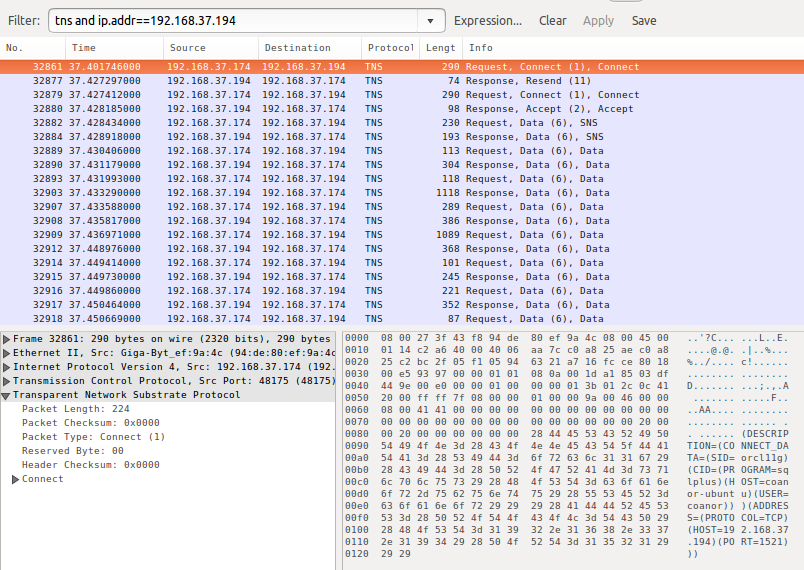
\includegraphics[width=\textwidth]{wireshark-tns.png}
\end{figure}

此处的过滤规则为 {\cf tns and ip.addr==192.168.37.194},其实,只要第一条即可,它限定了只显示与 TNS 协议相关的数据包。

图上列举的数据包中,来自一个 Oracle 的登陆操作。其中 174 作为客户端,194 作为服务器端,在第一条数据包中,{\ef Length} 列列出了数据包长度,{\ef Info} 列列出了是该数据包的详细信息,其中 {\cf Request} 指客户端请求服务器端,{\cf (1)} 是数据包类型,此处指一个 {\cf Connect} 操作。

在这条数据包中,从右下角的报文中可以看出,其中包含着一个 TNS 连接字符串,在该字符串中列举了连接的实例名 {\cf SID}、客户端工具为 {\cf sqlplus},客户端的主机名,使用的通信协议(TCP),客户端的 IP 以及连接的服务器端的端口。

左下角即是具体的数据包分析,Wireshark 目前只能识别部分 TNS 协议,比如连接数据包,对其他数据包,则只能识别头部数据,数据包后面的数据则不能识别。

对客户端发送出来的连接数据包而言,其中列举了包长度、校验和、包类型等等,图 \ref{fig:tns-connect} 中列出了 Wireshark 所分析出来的登陆数据包:

\begin{figure}[h!]
    \caption{Oracle 客户端发出的连接数据包}
    \label{fig:tns-connect}
    \centering
    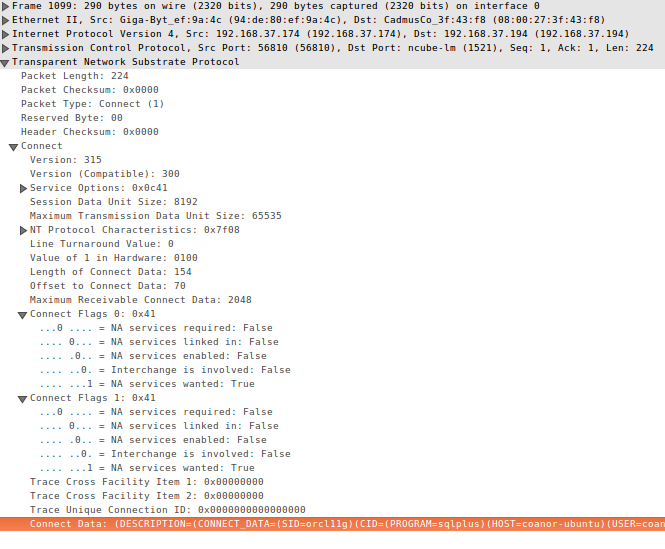
\includegraphics[width=\textwidth]{tns-connect.png}
\end{figure}

如果验证通过,服务器端会返回其 {\cf Accept} 数据包,Wireshark 的分析结果如图 \ref{fig:tns-accept} 所示:

\begin{figure}[h!]
    \caption{Oracle 服务器端发出的 Accept 数据包}
    \label{fig:tns-accept}
    \centering
    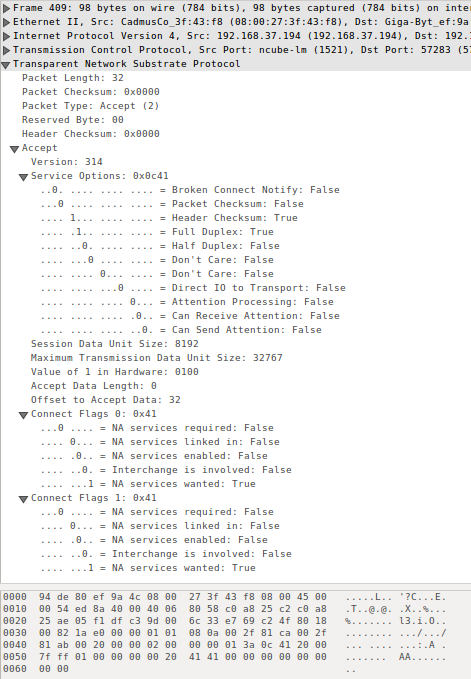
\includegraphics[width=0.8\textwidth]{tns-accept.png}
\end{figure}

连接建立以后,就可以发送 SQL 请求给服务器端,以下面的 SQL 语句为例:

\begin{lstlisting}[language=sql]
SELECT table_name FROM all_tables;
\end{lstlisting}

其 Wireshark 的分析结果如图 \ref{fig:tns-select} 所示:

\begin{figure}[h!]
    \caption{Oracle 的 SQL 查询语句数据包}
    \label{fig:tns-select}
    \centering
    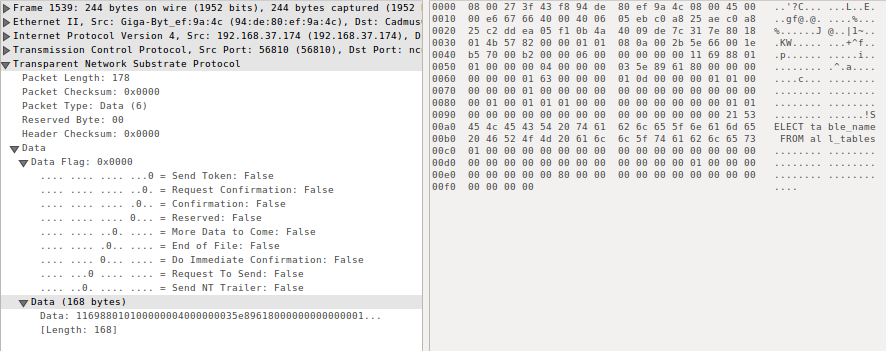
\includegraphics[width=\textwidth]{tns-select2.png}
\end{figure}

从右下角的报文可以看出,其中就包含有查询语句,但是从左下角 Wireshark 的报文分析来看,它并没有识别出该报文。而且经测试,同一条 SQL 语句,其报文结构{\bf 可能}不同,比如,再次输入上面的 SQL 语句,其报文如图 \ref{fig:tns-select-diff} 所示,此处再次列出上面的图片以做对比。\footnote{这种不同是有规律的,登陆后第一条查询语句的 payload 首字节为 {\cf 0x035e},后续的查询都是以 {\cf 0x1169}
开头,后面相隔固定字符之后再追加 {\cf 0x035e}。}

\begin{figure}[ht!]
    \caption{Oracle 中同一条 SQL 查询语句出来的数据包可能不同}
    \label{fig:tns-select-diff}
    \centering
    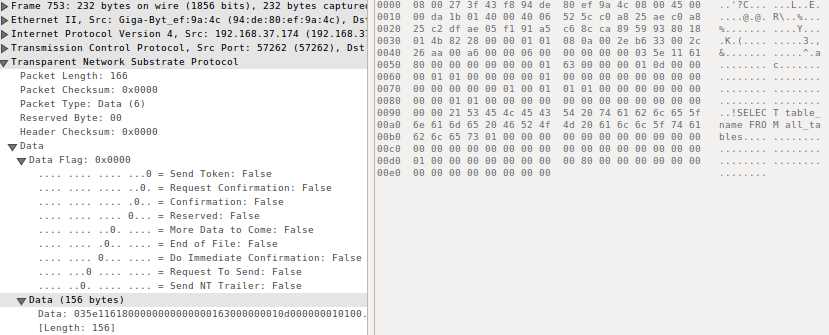
\includegraphics[width=\textwidth]{tns-select.png}
    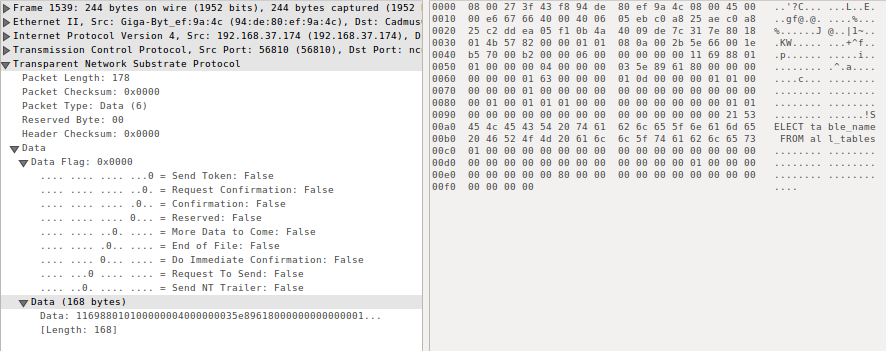
\includegraphics[width=\textwidth]{tns-select2.png}
\end{figure}

以上是 Oracle 数据库通信协议的 Wireshark 截图。下面再用 Wireshark 分析一下 MySQL 的通信数据包。

在 MySQL 的客户端与服务器端的通信过程中,先是服务器发送一个握手数据包,然后客户端再发送连接数据包。其通信过程如图 \ref{fig:mysql-comm-module} 所示:

\begin{figure}[h!]
    \caption{MySQL 的通信模型}
    \label{fig:mysql-comm-module}
    \centering
    
\includegraphics[width=0.3\textwidth]{mysql-flow.eps}
\end{figure}

\begin{figure}[h!]
    \caption{MySQL 服务器的握手数据包}
    \label{fig:mysql-server-hs}
    \centering
    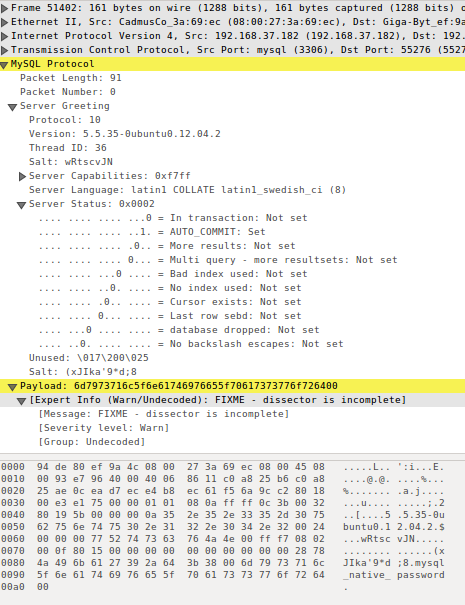
\includegraphics[width=0.5\textwidth]{mysql-server-hs.png}
\end{figure}

\begin{figure}[h!]
    \caption{MySQL 客户端的连接数据包}
    \label{fig:mysql-client-conn}
    \centering
    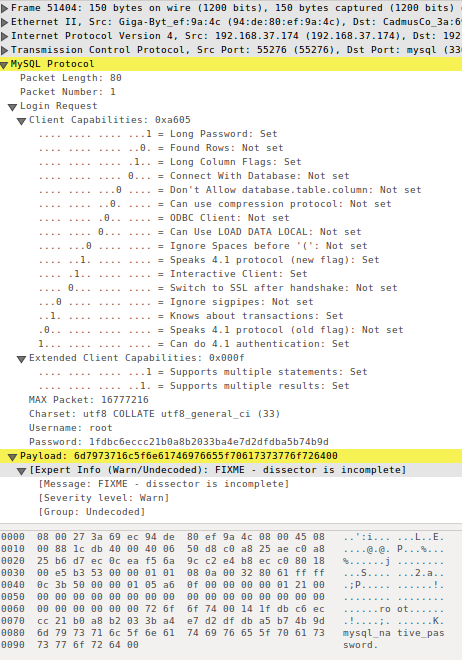
\includegraphics[width=0.5\textwidth]{mysql-client-conn.png}
\end{figure}

\begin{figure}[h!]
    \caption{MySQL 查询语句数据包}
    \label{fig:mysql-select}
    \centering
    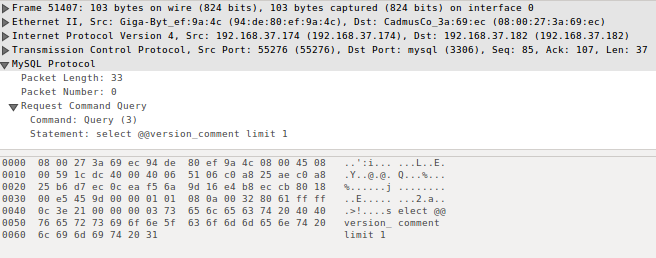
\includegraphics[width=0.5\textwidth]{mysql-select.png}
\end{figure}

Wireshark 能够完整地支持 Mysql 数据包解析,图 \ref{fig:mysql-server-hs} 中列举的是一个 MySQL 服务器发送的握手数据包。

然后是客户端的连接数据包,如图 \ref{fig:mysql-client-conn} 所示:

在 MySQL 的登陆过程中,会有一个 SQL 语句请求,在 Wireshark 中,其输出如图 \ref{fig:mysql-select} 所示:

另外的几种协议,比如 DB2 的 DADR 协议,SQL Server 的 TDS 协议,Wireshark 都有完整的支持,只需要按照 Wireshark 中的数据包分段即可将各种数据库的通信数据包抓取过来并进行分析。
